% apr lecture c'est quqnd même très très superficiel comme chapitre non ?


\chapter{Croissance en hauteur et en diamètre}

\begin{abstract}
Ce chapitre décrit comment l'activité des méristèmes est responsable de la croissance en hauteur et diamètre des arbres. Nous nous attarderons surtout à l'action du cambium, ou méristème secondaire, dont l'importance est fondamentale en sciences du bois. Il s'agit d'une fine couche de cellules dont la division est responsable de la formation des cellules de xylème et de phloème. La fin du chapitre montre comment l'action du cambium a une importance fondamentale sur la variabilité de la longueur des trachéides ou des fibres du centre de la tige vers l'écorce. Ces patrons de variabilité seront traités en détails dans les chapitres suivants. 
\end{abstract}

\minitoc

\section{Introduction}

La croissance des plantes ligneuses se produit selon deux mécanismes distincts, soit la croissance en hauteur et la croissance en diamètre. Chacun de ces mécanismes de croissance est assuré par des tissus particuliers appelés \textbf{méristèmes}. Les méristèmes sont des tissus embryonnaires \textbf{peu différenciés} et en constante division cellulaire. Ils produisent donc constamment de nouveaux tissus s'ajoutant à la plante.\\

On reconnait deux types de méristèmes dans les plantes ligneuses. Premièrement le \textbf{méristème apical} (ou méristème primaire) responsable de la croissance en hauteur et situé au bout des branches. Deuxièmement, \textbf{le cambium} (ou méristème secondaire) responsable de la croissance en diamètre et situé entre le xylème et le phloème.

\section{Méristème apical}

Le méristème apical est responsable de la croissance primaire, c'est-à-dire de l'élongation de la pousse terminale de la tige et des branches. Il produit trois types de tissus, le protoderme (ou épiderme), le procambium et le méristème de la moelle. Ces tissus évoluent vers le protoderme, le phloème secondaire, le cambium et le xylème secondaire. La Figure~\ref{fig:apical} montre chacune des étapes entre les deux. Comme l'objet de ce cours est d'abord relié à la croissance secondaire, vous pouvez vous contenter de retenir le rôle principal de ce méristème (vous n'avez pas à retenir chacune des étapes présentées à la Figure~\ref{fig:apical})

\begin{figure}[h]
	\centering
	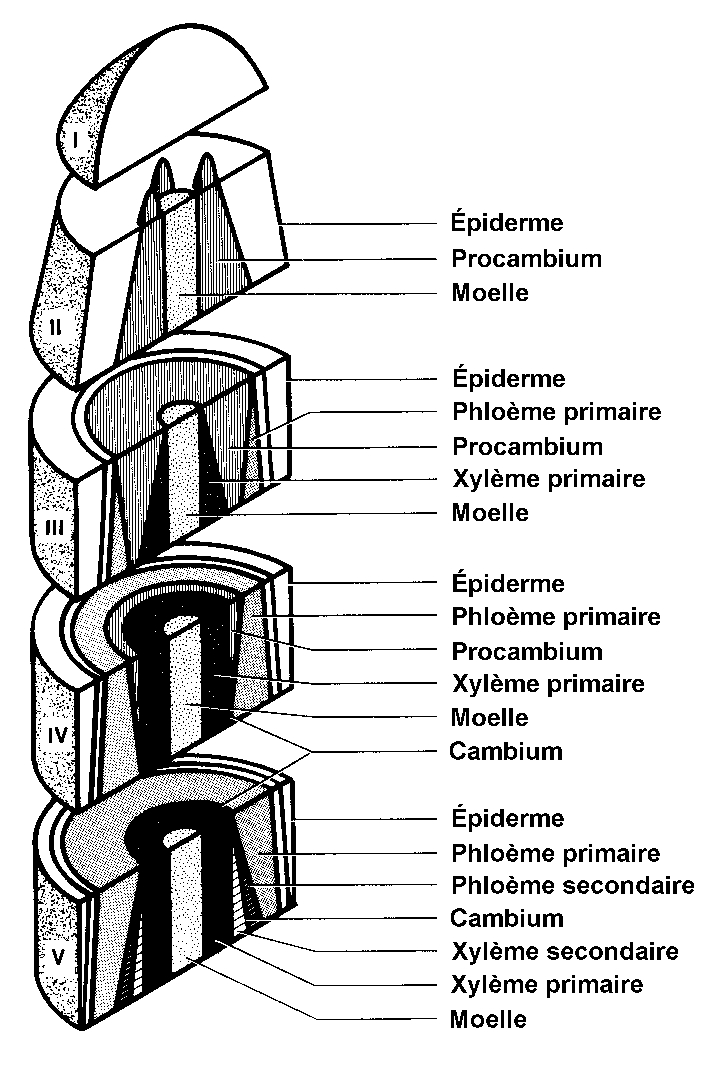
\includegraphics[scale=0.3]{img/ch5_apical}
	\caption{Représentation schématique du méristème apical (adapté de \cite{bowyer2007forest}).}
	\label{fig:apical}
\end{figure}.

\section{Cambium (méristème secondaire)}

Le cambium est une couche de cellules méristématiques en voie de division active située entre le xylème et le phloème (Figure~\ref{fig:camb_xyl}). Ces cellules sont appelées initiales du cambium. On retrouve deux types d'initiales du cambium, les \textbf{initiales fusiformes} et les \textbf{initiales de rayon}.

\begin{figure}[h]
	\centering
	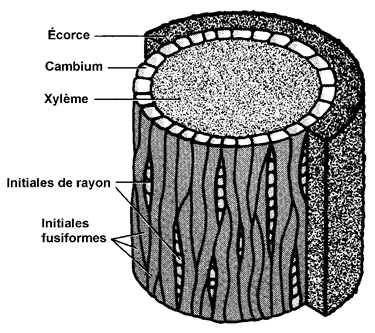
\includegraphics[scale=0.7]{img/ch5_camb_xyl}
	\caption{Représentation schématique du cambium, des initiales fusiformes et des initiales de rayon (adapté de \cite{bowyer2007forest}).}
\label{fig:camb_xyl}
\end{figure}

\subsection{Initiales fusiformes}

Les initiales fusiformes donnent naissance aux cellules longitudinales autant du côté du xylème que du phloème. En plan LT, les initiales fusiformes ont une forme aplatie et effilée (Figure~\ref{fig:camb_xyl}) alors qu'elles ont un profil en fuseau dans le plan LR (Figure~\ref{fig:periclinal}). Elles sont d'une longueur variant de 2 à 9 mm et d'un diamètre de 30 µm et plus chez les résineux. Chez les feuillus, les initiales fusiformes ont une longueur variant de 0,3 à 2 mm.\\

Le cambium étagé est un cas particulier que l'on rencontre chez certaines espèces incluant l'acacia blanc (\textit{Robinia pseudoacacia}). Chez ces bois, les initiales fusiformes sont de longueur plus ou moins uniforme et sont groupées en rangées horizontales (Figure~\ref{fig:cambium_etage}).  La longueur des initiales fusiformes chez les bois à cambium étagé varie de 140 µm à 520 µm.

\begin{figure}[h]
	\centering
	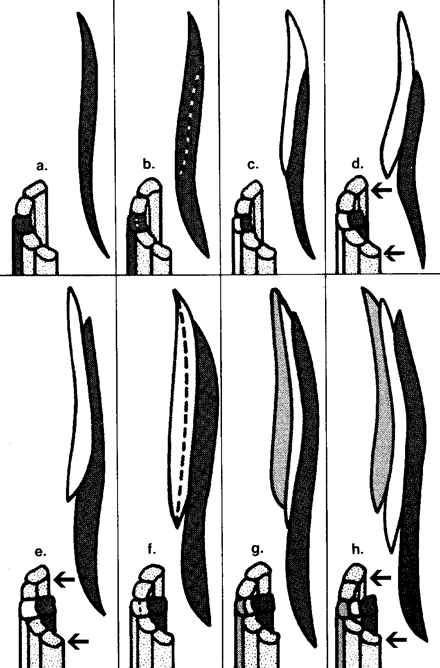
\includegraphics[scale=0.5]{img/ch5_periclinal}
	\caption{Cloisonnement périclinal des initiales fusiformes du cambium (adapté de \cite{bowyer2007forest}).}
	\label{fig:periclinal}
\end{figure}

\begin{figure}[h]
	\centering
	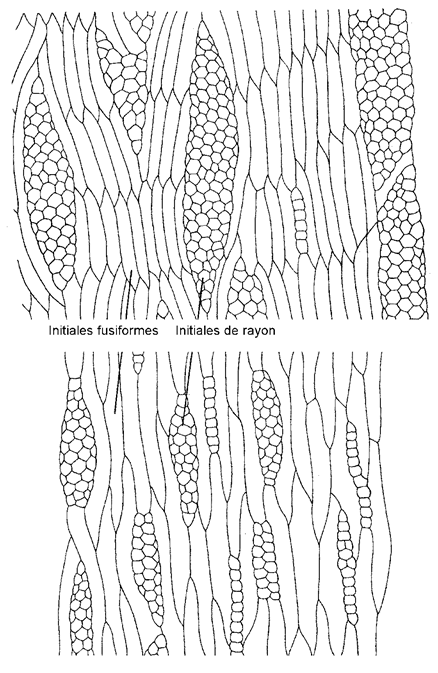
\includegraphics[scale=0.4]{img/ch5_cambium_etage}
	\caption{Cambium en plan LT.  1) cambium étagé, 2) cambium non-étagé (adapté de \cite{fahn1990plant}).}
\label{fig:cambium_etage}
\end{figure}

\subsection{Initiales de rayon}

Les initiales de rayon sont des cellules de forme cubique donnant naissance aux cellules de rayon et aux cellules épithéliales (Figures~\ref{fig:cambium_etage}~et~\ref{fig:cellules_resume}). La Figure~\ref{fig:cellules_resume} peut vous servir de résumé des chapitres sur l'anatomie du bois des \hyperref[resineux]{résineux} et des \hyperref[feuillus]{feuillus}.

\subsubsection{Processus de division cellulaire dans le cambium}

Les cellules du cambium peuvent se diviser successivement pour former de nouvelles initiales du cambium et de nouvelles cellules de xylème et de phloème.  Les initiales du cambium se divisent selon deux mécanismes différents : 1) selon un cloisonnement \textbf{périclinal} et 2) selon un cloisonnement \textbf{anticlinal}.

\begin{figure}[h]
\centering
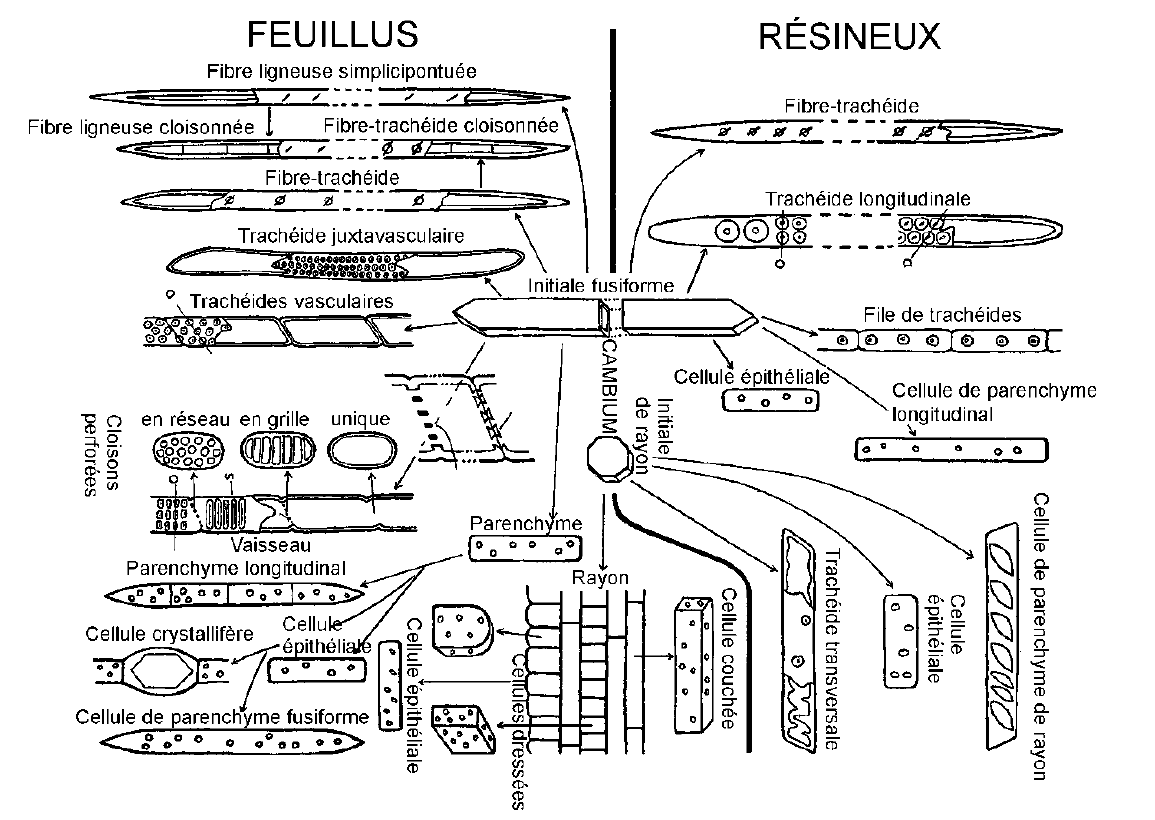
\includegraphics[width=1\textwidth]{img/ch5_cellules_resume}
\caption{Types de cellules du xylème produites par les initiales du cambium chez les résineux et les feuillus (adapté de \cite{jane1970structure}).}
\label{fig:cellules_resume}
\end{figure}

\subsubsection{Cloisonnement périclinal}

Le cloisonnement périclinal s'effectue selon un plan LT tel qu'illustré aux Figures~\ref{fig:periclinal}, \ref{fig:peri_anti} et \ref{fig:peri_anti_haut}. Ce type de cloisonnement permet la croissance en diamètre de la tige par la formation de nouvelles cellules de xylème et de phloème.

\begin{figure}[h]
\centering
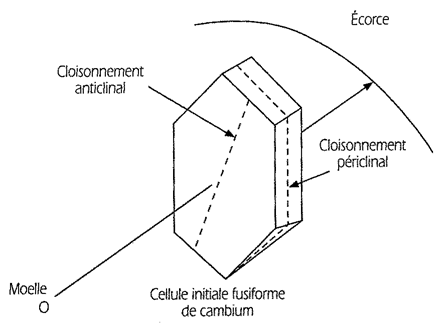
\includegraphics[scale=0.8]{img/ch5_peri_anti}
\caption{Cloisonnement périclinal et anticlinal d'une initiale fusiforme du cambium (d'après \cite{doucet2009manuel}).}
\label{fig:peri_anti}
\end{figure}

\begin{figure}[h]
\centering
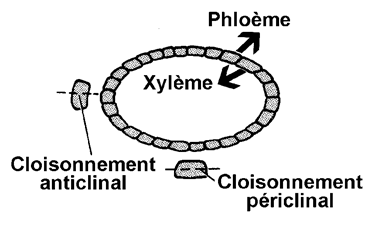
\includegraphics[scale=0.5]{img/ch5_peri_anti_haut}
\caption{Cloisonnement périclinal et anticlinal d'une initiale du cambium (adapté de \cite{bowyer2007forest}).}
\label{fig:peri_anti_haut}
\end{figure}

\subsubsection{Cloisonnement anticlinal}

Le cloisonnement anticlinal s'effectue selon un plan LR tel qu'illustré aux Figures~\ref{fig:peri_anti} et \ref{fig:peri_anti_haut}. Il est responsable de la formation de nouvelles cellules du cambium permettant la croissance en circonférence de ce dernier. Il faut remarquer que la croissance en circonférence du cambium est également due à la croissance subséquente des initiales du cambium en hauteur et en diamètre suite à la division cellulaire tel qu'illustré à la Figure~\ref{fig:elongation}.\\

La production de nouvelles initiales de rayon a lieu selon différents mécanismes.  Elles peuvent être produites par la réduction en longueur d'un certain nombre d'initiales fusiformes ou par la division cellulaire d'initiales fusiformes ou de parties d'initiales fusiformes tel qu'illustré à la Figure~\ref{fig:init_rayons}. Dans le cas des feuillus à rayons plurisériés, le nombre d'initiales de rayons augmente par division des initiales de rayon présentes ou par fusion de plusieurs rayons voisins.\\

\begin{figure}[h]
\centering
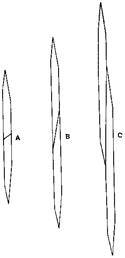
\includegraphics[scale=0.7]{img/ch5_elongation}
\caption{Cloisonnement anticlinal et allongement des initiales fusiformes du cambium. A) l'initiale se divise selon un cloisonnement anticlinal, B) et C) les deux cellules ainsi produites s'allongent (d'après \cite{jane1970structure}).}
\label{fig:elongation}
\end{figure}

\begin{figure}[h]
\centering
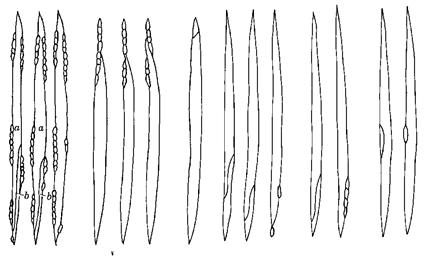
\includegraphics[scale=0.7]{img/ch5_init_rayons}
\caption{Formation des initiales de rayon à partir des initiales fusiformes (d'après \cite{panshin1980textbook}).}
\label{fig:init_rayons}
\end{figure}

\subsection{Mécanisme de formation des cellules de xylème et de phloème}

La croissance de l'arbre en diamètre est causée par le cloisonnement périclinal des initiales fusiformes et des initiales de rayon. Ces cloisonnements peuvent produire soit une nouvelle initiale de cambium et une cellule-mère de xylème, soit une nouvelle initiale de cambium et une cellule-mère de phloème. Les cellules-mères de xylème sont produites plus fréquemment que les cellules-mères de phloème. Une cellule-mère de phloème se divisera en deux cellules de phloème alors qu'une cellule-mère de xylème se divisera en deux cellules-filles de xylème qui se diviseront à nouveau chacune en deux cellules de xylème. On obtient comme résultat qu'une division par cloisonnement périclinal de l'initiale de cambium résulte en deux nouvelles cellules de phloème ou quatre nouvelles cellules de xylème.  De plus, un moins grand nombre de divisions de l'initiale de cambium donnent naissance à une cellule-mère de phloème. Ceci explique que le cambium produit beaucoup plus de cellules de xylème que de phloème. Le mécanisme général de formation des cellules de xylème et de phloème est présenté aux Figures~\ref{fig:xyl_phlo} et \ref{fig:xyl_phlo_img}.

\subsection{Variation de la longueur des initiales fusiformes du cambium}

La longueur des initiales fusiformes du cambium varie en fonction d'un certain nombre de facteurs. En règle générale, la longueur des initiales fusiformes détermine la longueur des cellules du xylème et du phloème.  De plus, la longueur des initiales fusiformes est inversement proportionnelle au taux de cloisonnement anticlinal. Ceci implique que plus le taux de croissance est élevé, plus les initiales fusiformes sont courtes.

\begin{figure}[h]
\centering

\begin{tikzpicture}[level distance=1.9in,sibling distance=.2in,scale=.75]
\tikzset{edge from parent/.style= 
            {thick, draw,
                edge from parent fork right},every tree node/.style={draw,minimum width=1in,text width=1.5in, align=center},grow'=right}
\Tree 
    [. {Initiale de cambium}
        [.{Cellule-mère phloème}
            [.{Cellule de phloème} ]
            [.{Cellule de phloème} ]
        ]
        [.{Cellule-mère xylème}
            [.{Cellule fille de xylème} 
            	[. {Cellule de xylème} ] 
            	[. {Cellule de xylème} ] ]
            [.{Cellule fille de xylème} 
                 [. {Cellule de xylème} ] 
                 [. {Cellule de xylème} ] ]
        ] 
    ]
\end{tikzpicture}
\caption{Mécanisme de formation des cellules de xylème et de phloème}
\label{fig:xyl_phlo}	
\end{figure}


\begin{figure}[h]
\centering
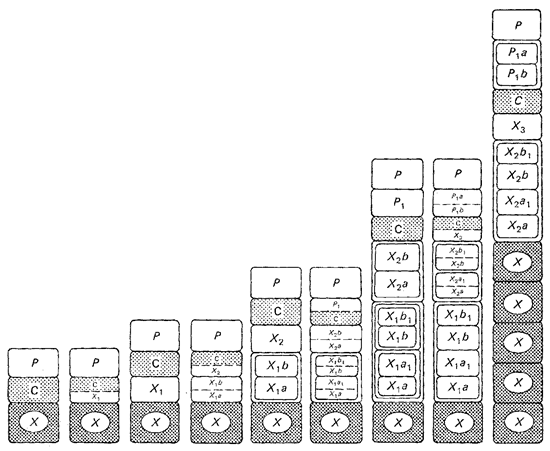
\includegraphics[scale=0.8]{img/ch5_develop_cambium}
\caption{Mécanisme de formation des cellules de xylème et de phloème (adapté de \cite{panshin1980textbook}).}
\label{fig:xyl_phlo_img}
\end{figure}
%
%
\subsubsection{Effet de la distance radiale de la moelle vers l'écorce}

La longueur des initiales fusiformes augmente de la moelle vers l'écorce comme le montre la Figure~\ref{fig:cloisonnement_long}. De plus, la proportion des initiales fusiformes subissant un cloisonnement anticlinal diminue de la moelle vers l'écorce.

\subsubsection{Effet de la hauteur dans l'arbre}

La longueur des initiales fusiformes augmente de la souche à la base de la cime vivante et décroît jusqu'au sommet de l'arbre.

\subsubsection{Effet du taux de croissance}\label{prt_longueur}

Une augmentation du taux de croissance implique un accroissement du nombre de cloisonnements anticlinaux, donc une réduction de la longueur des initiales fusiformes.

\begin{figure}[h]
\centering
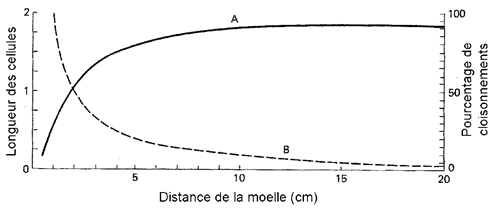
\includegraphics[scale=0.7]{img/ch5_cloisonnement_long}
\caption{Changements des initiales fusiformes en fonction de leur position par rapport à la moelle. A: Longueur des initiales fusiformes, B: Pourcentage d'initiales fusiformes effectuant un cloisonnement anticlinal (adapté de \cite{panshin1980textbook}).}
\label{fig:cloisonnement_long}
\end{figure}

\section{Mécanisme de croissance des cellules}

Le mécanisme de croissance des cellules du bois à partir des divisons périclines des initiales fusiformes du cambium est illustré à la Figure \ref{fig:mecacroissance}.

\begin{figure}[h]
	\centering
	
	\begin{tikzpicture}[level distance=1cm, text width=6cm, align=center]
	\node[draw] {Initiale fusiforme}
	child {node[draw] {Cellule-mère (1)}
		child {node[draw] {Cellules filles (2)} 
			child {node[draw] {Cellules de xylème (4)} 
				child[level distance=1.3cm] {node[draw] {Développement (croissance) \\ {\scriptsize Longueur, diamètre, LM, P ; pectine et pas de lignine}} 
					child {node[draw](cr){Croissance de la paroi secondaire \\ {\scriptsize Le jour, formation de S\sub{1}, S\sub{2} et S\sub{3}}} 
						child {node[draw](li){Lignification de la paroi cellulaire \\ {\scriptsize La nuit}} 
							child[level distance=1cm] {node[draw] {Mort du protoplasme et dépôt sur S\sub{3}} } } } } } }
	};
	
	\draw[semithick,->] (li)..controls +(east:4) and +(east:4)..(cr);
	\end{tikzpicture}
	
	\caption{Mécanisme de croissance des cellules du bois à partir des divisons périclinales des initiales fusiformes du cambium.}
	\label{fig:mecacroissance}
\end{figure}

\subsection{Activité du cambium vasculaire selon la saison}

Le cambium est inactif en hiver. Au printemps, l'activité du cambium reprend si la température moyenne demeure supérieure à 5°C pour une semaine. La reprise de l'activité du cambium coïncide avec la production d'auxines par les méristèmes apicaux lors de l'ouverture des bourgeons. À l'automne, l'arrêt de l'activité du cambium est fonction de la photopériode.
%
%
%Références
%
%Benabdallah, B. 1996. Structure de la matière ligneuse.  Manuel de foresterie.  Ordre des ingénieurs forestiers du Québec et Presses de l'Université Laval. pp. 1276-1296. 
%Fahn, A. 1990.  Plant anatomy.  Fourth edition.  Pergamon Press, Oxford.  588 p.
%Jane, F.W. 1970. The structure of wood.  Second Edition.  Adam and Charles Black, London.  478 p.
%Panshin, A.J.; de Zeeuw, C. 1980.  Textbook of wood technology.  Fourth edition.  McGraw-Hill Book Co. New York.  722 p.
